\documentclass[aspectratio=169,12pt]{beamer}
\usepackage[utf8]{inputenc}
\usepackage{amsmath, amssymb}
\usepackage{booktabs}
\usepackage{colortbl}
\usepackage{hyperref}
\usepackage{makecell}
\usepackage{ragged2e}
\usepackage{tikz}
\usetikzlibrary{arrows.meta, positioning, shapes.geometric, calc, tikzmark, shapes.misc, fit, decorations.pathreplacing}
\usepackage[siunitx, RPvoltages]{circuitikz}
\usepackage{tcolorbox}
\usepackage{array}
\usetheme{Madrid}

% Custom colors
\definecolor{correctgreen}{RGB}{0,150,0}
\definecolor{incorrectred}{RGB}{200,0,0}
\definecolor{counterblue}{RGB}{70,130,255}
\definecolor{highlightyellow}{RGB}{255,230,100}

\title{Branch Prediction}
\author{Computer Architecture 2340267}
\date{2025, Recitation \#6}
\begin{document}

\frame{\titlepage}

%==========================================
\begin{frame}{2-Bit Counter Prediction (Threshold of 2)}
\vspace{-0.3cm}

% \begin{tikzpicture}[
%     every node/.style={font=\footnotesize},
%     pattern/.style={minimum width=0.5cm, minimum height=0.5cm, draw=black!60},
%     predict/.style={minimum width=0.5cm, minimum height=0.5cm, draw=black!60},
%     counter/.style={minimum width=0.5cm, minimum height=0.5cm, draw=counterblue, text=counterblue},
%     correct/.style={fill=correctgreen!20},
%     wrong/.style={fill=incorrectred!30},
%     arrow/.style={->, thick, >=stealth}
% ]

% % Labels
% \node[anchor=east] at (-0.5, 0) {\textbf{Pattern:}};
% \node[anchor=east] at (-0.5, -1) {\textbf{2-bit Prediction:}};
% \node[anchor=east] at (-0.5, -2) {\textbf{Counter:}};

% % Pattern row
% \foreach \i in {0,...,19} {
%     \pgfmathtruncatemacro{\val}{mod(\i,5) < 4 ? 1 : 0}
%     \pgfmathtruncatemacro{\groupnum}{floor(\i/5)}
%     \node[pattern, fill=\val ? white : gray!20] (p\i) at (\i*0.6, 0) {\val};
% }
% \node at (20*0.6, 0) {...};

\begin{tikzpicture}[
    every node/.style={font=\footnotesize},
    pattern/.style={minimum width=0.5cm, minimum height=0.5cm, draw=black!60},
    predict/.style={minimum width=0.5cm, minimum height=0.5cm, draw=black!60},
    counter/.style={minimum width=0.5cm, minimum height=0.5cm, draw=blue},
    correct/.style={fill=green!20},
    wrong/.style={fill=red!30},
    arrow/.style={->, thick, >=stealth}
]

% Labels
\node[anchor=east] at (-0.5, 0) {\textbf{Pattern:}};
\node[anchor=east] at (-0.5, -1) {\textbf{2-bit Prediction:}};
\node[anchor=east] at (-0.5, -1.6) {\textbf{Counter:}};

% Pattern row
\foreach \i in {0,...,19} {
    \pgfmathtruncatemacro{\val}{mod(\i,5) < 4 ? 1 : 0}
    \pgfmathtruncatemacro{\groupnum}{floor(\i/5)}
    \ifnum\val=1
        \node[pattern, fill=white] (p\i) at (\i*0.6, 0) {\val};
    \else
        \node[pattern, fill=gray!20] (p\i) at (\i*0.6, 0) {\val};
    \fi
}
\node at (20*0.6, 0) {...};

% Prediction row
\foreach \i in {0,...,19} {
    \node[predict] (pred\i) at (\i*0.6, -1) {1};
}
\node at (20*0.6, -1) {...};

% Counter row
\foreach \i in {0,...,19} {
    \pgfmathtruncatemacro{\posInGroup}{mod(\i,5)}
    \ifnum\posInGroup=0
        \node[counter, color=blue] (c\i) at (\i*0.6, -1.6) {2};
    \else
        \ifnum\posInGroup=4
            \node[counter, color=blue] (c\i) at (\i*0.6, -1.6) {2};
        \else
            \node[counter, color=blue] (c\i) at (\i*0.6, -1.6) {3};
        \fi
    \fi
}

% Misprediction indicators
\foreach \i in {4,9,14,19} {
    % Highlight mispredicted positions
    \node[predict, wrong] at (\i*0.6, -1) {1};
    \draw[red, ultra thick] (p\i.south west) -- (p\i.south east);
    \draw[red, ultra thick] (pred\i.north west) -- (pred\i.north east);
    
    % Add X mark for misprediction
    \node[color=red, font=\Large] at (\i*0.6, -0.5) {$\times$};
}
% Correct prediction indicators (check marks)
\foreach \i in {0,1,2,3,5,6,7,8,10,11,12,13,15,16,17,18} {
    \node[color=green!60!black, font=\small] at (\i*0.6, -0.5) {$\checkmark$};
}
% Group brackets
\foreach \g in {0,1,2,3} {
    \pgfmathtruncatemacro{\startx}{\g*5}
    \pgfmathtruncatemacro{\endx}{\g*5+4}
    \pgfmathtruncatemacro{\gnum}{\g+1}
    \draw[decoration={brace,amplitude=5pt,mirror}, decorate, thick, gray] 
        (\startx*0.6-0.25, -2.0) -- (\endx*0.6+0.25, -2.0);
    \node[gray] at (\startx*0.6+1.2, -2.4) {iteration \gnum};
}

\end{tikzpicture}

\vspace{-0.2cm}
\begin{alertblock}{Key Observation}
\centering
\textcolor{incorrectred}{\textbf{2-bit counter $\rightarrow$ one misprediction every iteration}}
\end{alertblock}

\vspace{-0.2cm}
\begin{block}{Performance Example}
\scriptsize
\begin{columns}[T]
\column{0.55\textwidth}
\begin{itemize}
\item Assume 1 of 20 branches mispredicts\\
%      \textcolor{gray}{(19 predictions are correct)}
\item Branch frequency: 20\% \textcolor{gray}{(1 of 5 instructions)}
\item[] \textcolor{incorrectred}{\textbf{$\rightarrow$ 1 mispredict every 100 instructions}}
\item IPC without penalty = 2\\
\end{itemize}

\column{0.45\textwidth}
\begin{itemize}
%      \textcolor{gray}{(two instructions finish per cycle)}
\item Mispredict penalty: 10 cycles
\item[] \textcolor{incorrectred}{\textbf{$\rightarrow$ 1 mispredict every 50 cycles}}
\item[] \textcolor{incorrectred}{\textbf{$\rightarrow$ 10 cycles penalty every 50 cycles}}
\item[] \textcolor{incorrectred}{\textbf{$\rightarrow$ 20\% performance loss!}}
\end{itemize}
\end{columns}
\end{block}

\end{frame}

\begin{frame}{Better Idea: Use Branch History}

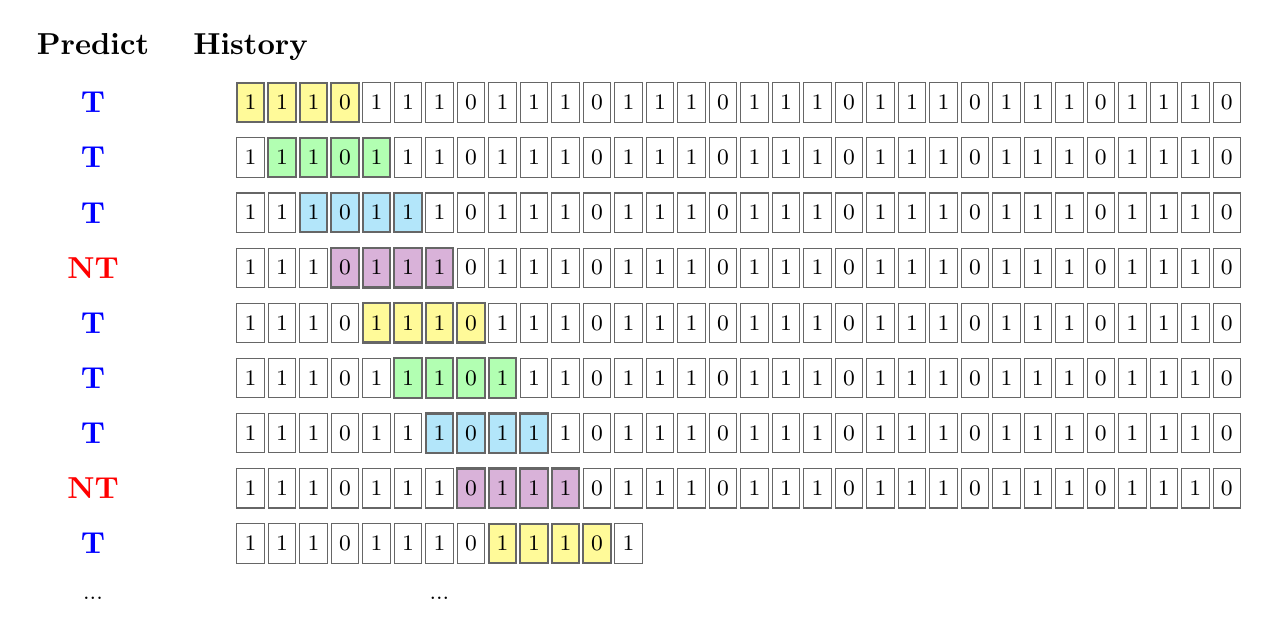
\begin{tikzpicture}[
    every node/.style={font=\footnotesize},
    bit/.style={minimum width=0.35cm, minimum height=0.5cm, inner sep=1pt, draw=black!60},
    history1110/.style={bit, fill=yellow!40, thick},
    history1101/.style={bit, fill=green!30, thick},
    history1011/.style={bit, fill=cyan!30, thick},
    history0111/.style={bit, fill=violet!30, thick},
    predict/.style={font=\fontsize{11}{13}\selectfont\bfseries, minimum width=1cm},
    label/.style={font=\fontsize{11}{13}\selectfont\bfseries}
]

% Labels positioned using relative positioning
\node[label, text height=1.5ex, text depth=.25ex] (predict_label) at (0, 0) {Predict};
\node[label, text height=1.5ex, text depth=.25ex] (history_label) at (2, 0) {History};

% Pattern template (repeated pattern: 11101110...)
\def\patternseq{1,1,1,0,1,1,1,0,1,1,1,0,1,1,1,0,1,1,1,0,1,1,1,0,1,1,1,0,1,1,1,0}

% Define row spacing
\def\rowspacing{0.7}

% Row 1 - History: 1110 -> Predict T
\node[predict, text=blue] (pred1) at (0, -1*\rowspacing) {T};
\foreach \i in {0,...,31} {
    \pgfmathparse{{\patternseq}[\i]}
    \pgfmathtruncatemacro{\val}{\pgfmathresult}
    \ifnum\i<4
        \node[history1110] at (2 + \i*0.4, -1*\rowspacing) {\val};
    \else
        \node[bit] at (2 + \i*0.4, -1*\rowspacing) {\val};
    \fi
}

% Row 2 - History: 1101 -> Predict T
\node[predict, text=blue] (pred2) at (0, -2*\rowspacing) {T};
\foreach \i in {0,...,31} {
    \pgfmathparse{{\patternseq}[\i]}
    \pgfmathtruncatemacro{\val}{\pgfmathresult}
    \ifnum\i>0 \ifnum\i<5
        \node[history1101] at (2 + \i*0.4, -2*\rowspacing) {\val};
    \else
        \node[bit] at (2 + \i*0.4, -2*\rowspacing) {\val};
    \fi \fi
    \ifnum\i=0
        \node[bit] at (2 + \i*0.4, -2*\rowspacing) {\val};
    \fi
}

% Row 3 - History: 1011 -> Predict T  
\node[predict, text=blue] (pred3) at (0, -3*\rowspacing) {T};
\foreach \i in {0,...,31} {
    \pgfmathparse{{\patternseq}[\i]}
    \pgfmathtruncatemacro{\val}{\pgfmathresult}
    \ifnum\i>1 \ifnum\i<6
        \node[history1011] at (2 + \i*0.4, -3*\rowspacing) {\val};
    \else
        \node[bit] at (2 + \i*0.4, -3*\rowspacing) {\val};
    \fi \fi
    \ifnum\i<2
        \node[bit] at (2 + \i*0.4, -3*\rowspacing) {\val};
    \fi
}

% Row 4 - History: 0111 -> Predict NT
\node[predict, text=red] (pred4) at (0, -4*\rowspacing) {NT};
\foreach \i in {0,...,31} {
    \pgfmathparse{{\patternseq}[\i]}
    \pgfmathtruncatemacro{\val}{\pgfmathresult}
    \ifnum\i>2 \ifnum\i<7
        \node[history0111] at (2 + \i*0.4, -4*\rowspacing) {\val};
    \else
        \node[bit] at (2 + \i*0.4, -4*\rowspacing) {\val};
    \fi \fi
    \ifnum\i<3
        \node[bit] at (2 + \i*0.4, -4*\rowspacing) {\val};
    \fi
}

% Row 5 - History: 1110 -> Predict T
\node[predict, text=blue] (pred5) at (0, -5*\rowspacing) {T};
\foreach \i in {0,...,31} {
    \pgfmathparse{{\patternseq}[\i]}
    \pgfmathtruncatemacro{\val}{\pgfmathresult}
    \ifnum\i>3 \ifnum\i<8
        \node[history1110] at (2 + \i*0.4, -5*\rowspacing) {\val};
    \else
        \node[bit] at (2 + \i*0.4, -5*\rowspacing) {\val};
    \fi \fi
    \ifnum\i<4
        \node[bit] at (2 + \i*0.4, -5*\rowspacing) {\val};
    \fi
}

% Row 6 - History: 1101 -> Predict T
\node[predict, text=blue] (pred6) at (0, -6*\rowspacing) {T};
\foreach \i in {0,...,31} {
    \pgfmathparse{{\patternseq}[\i]}
    \pgfmathtruncatemacro{\val}{\pgfmathresult}
    \ifnum\i>4 \ifnum\i<9
        \node[history1101] at (2 + \i*0.4, -6*\rowspacing) {\val};
    \else
        \node[bit] at (2 + \i*0.4, -6*\rowspacing) {\val};
    \fi \fi
    \ifnum\i<5
        \node[bit] at (2 + \i*0.4, -6*\rowspacing) {\val};
    \fi
}

% Row 7 - History: 1011 -> Predict T
\node[predict, text=blue] (pred7) at (0, -7*\rowspacing) {T};
\foreach \i in {0,...,31} {
    \pgfmathparse{{\patternseq}[\i]}
    \pgfmathtruncatemacro{\val}{\pgfmathresult}
    \ifnum\i>5 \ifnum\i<10
        \node[history1011] at (2 + \i*0.4, -7*\rowspacing) {\val};
    \else
        \node[bit] at (2 + \i*0.4, -7*\rowspacing) {\val};
    \fi \fi
    \ifnum\i<6
        \node[bit] at (2 + \i*0.4, -7*\rowspacing) {\val};
    \fi
}

% Row 8 - History: 0111 -> Predict NT
\node[predict, text=red] (pred8) at (0, -8*\rowspacing) {NT};
\foreach \i in {0,...,31} {
    \pgfmathparse{{\patternseq}[\i]}
    \pgfmathtruncatemacro{\val}{\pgfmathresult}
    \ifnum\i>6 \ifnum\i<11
        \node[history0111] at (2 + \i*0.4, -8*\rowspacing) {\val};
    \else
        \node[bit] at (2 + \i*0.4, -8*\rowspacing) {\val};
    \fi \fi
    \ifnum\i<7
        \node[bit] at (2 + \i*0.4, -8*\rowspacing) {\val};
    \fi
}

% Row 9 - History: 1110 -> Predict T
\node[predict, text=blue] (pred9) at (0, -9*\rowspacing) {T};
\foreach \i in {0,...,12} {
    \pgfmathparse{{\patternseq}[\i]}
    \pgfmathtruncatemacro{\val}{\pgfmathresult}
    \ifnum\i>7 \ifnum\i<12
        \node[history1110] at (2 + \i*0.4, -9*\rowspacing) {\val};
    \else
        \node[bit] at (2 + \i*0.4, -9*\rowspacing) {\val};
    \fi \fi
    \ifnum\i<8
        \node[bit] at (2 + \i*0.4, -9*\rowspacing) {\val};
    \fi
}

% ... dots
\node at (0, -10*\rowspacing) {...};
\node at (2 + 6*0.4, -10*\rowspacing) {...};

\end{tikzpicture}

\end{frame}

%==========================================
\definecolor{correctgreen}{RGB}{0,150,0}
\definecolor{incorrectred}{RGB}{200,0,0}
\definecolor{counterblue}{RGB}{70,130,255}
\definecolor{highlightyellow}{RGB}{255,230,100}
\definecolor{codeblue}{RGB}{0,0,200}

% Command to highlight state changes
\newcommand{\stateHighlight}[2]{%
  \ifnum#1=1
    \cellcolor{highlightyellow}#2%
  \else
    #2%
  \fi
}

% Macro for BHR display as boxes
\newcommand{\BHRbox}[4]{%
  \begin{tikzpicture}[baseline=(current bounding box.center)]
    \foreach \bit [count=\i] in {#1,#2,#3,#4} {
      \node[draw, minimum width=6mm, minimum height=5mm, inner sep=1pt] at (\i*0.7,0) {\footnotesize\bit};
    }
  \end{tikzpicture}
}

% Helper to expand stored BHR and pass to BHRbox
\newcommand{\BHRboxFromStorage}[4]{%
  % Direct storage of 4 values
  \BHRbox{#1}{#2}{#3}{#4}%
}

% Helper for pgfkeys stored BHR
\newcommand{\BHRdisplay}[1]{%
  % #1 contains {b1}{b2}{b3}{b4}
  % We need to extract these values
  \expandafter\BHRdisplayHelper#1%
}
\newcommand{\BHRdisplayHelper}[4]{%
  \BHRbox{#1}{#2}{#3}{#4}%
}

% Setup pgfkeys for local frame parameters
\pgfkeys{
  /localframe/.cd,
  ip/.store in=\localframeIP,
  ip/.default={},
  outcome/.store in=\localframeOutcome,
  bhr1/.code={\def\localframeBHROne{#1}},
  bhr2/.code={\def\localframeBHRTwo{#1}},
  bhr3/.code={\def\localframeBHRThree{#1}},
  r1/.store in=\localframeROne,
  r2/.store in=\localframeRTwo,
  r3/.store in=\localframeRThree,
  states/.store in=\localframeStates,
  description/.store in=\localframeDesc,
  % Set defaults - don't set BHR defaults, they cause issues
  ip={},
  outcome={},
  % bhr1={0}{0}{0}{0},  % Don't set default
  % bhr2={0}{0}{0}{0},  % Don't set default
  % bhr3={0}{0}{0}{0},  % Don't set default
  r1={0},
  r2={0},
  r3={0},
  states={},
  description={},
}


\begin{frame}
  \frametitle{Code Example}
  
  \begin{columns}[T]
    \column{0.42\textwidth}
    \centering
    \textbf{C Code}
    \vspace{0.5em}
    
    \begin{tcolorbox}[colback=white, colframe=black!60, boxrule=0.8pt, left=3pt, right=3pt, top=3pt, bottom=3pt]
      \small\ttfamily
      \begin{tabbing}
      \hspace{1em}\=\hspace{1em}\=\kill
      \colorbox{red!25}{for (i=100; i>0; i--)}\\ 
      \> \colorbox{green!25}{for (j=2; j<5; j++)}\\
      \> \> \colorbox{cyan!25}{if (i\%j == 0)} \{\\
      \> \>   \colorbox{gray!15}{. . .}\\
      \> \> \}\\
      \end{tabbing}
    \end{tcolorbox}
    
    \column{0.58\textwidth}
    \centering
    \textbf{Assembly}
    \vspace{0.5em}
    
    \begin{tcolorbox}[colback=white, colframe=black!60, boxrule=0.8pt, left=3pt, right=3pt, top=3pt, bottom=3pt]
      \small\ttfamily
      \renewcommand{\arraystretch}{1.1}
      \begin{tabular}{@{}r@{~~}l@{}}
        & \colorbox{green!25}{Addi~~~r5, r0, 5}\\
        & \colorbox{red!25}{Addi~~~r1, r0, 100}\\
        L1: & \colorbox{green!25}{Addi~~~r2, r0, 2}\\
        L2: & \colorbox{cyan!25}{Mod~~~~r3, r1, r2}\\
        & \colorbox{cyan!25}{Bne~~~~r3, r0, IF}\\
        & \colorbox{gray!15}{. . .}\\
        IF: & \colorbox{green!25}{Addi~~~r2, r2, 1}\\
        & \colorbox{green!25}{Bne~~~~r2, r5, L2}\\
        & \colorbox{red!25}{Subi~~~r1, r1, 1}\\
        & \colorbox{red!25}{Bne~~~~r1, r0, L1}\\
      \end{tabular}
    \end{tcolorbox}
  \end{columns}
  
  \vspace{0.8em}
  
  \begin{center}
    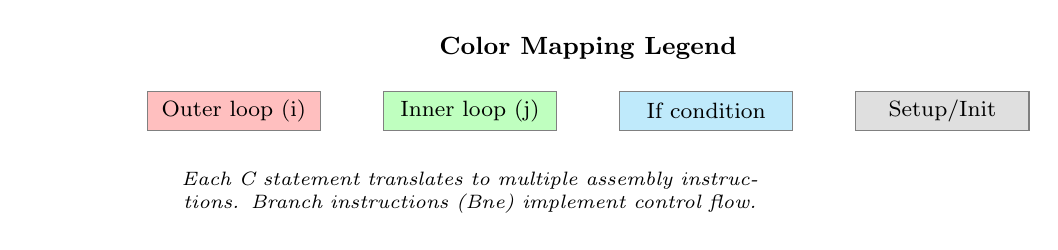
\begin{tikzpicture}[
      legend/.style={draw=black!50, minimum width=2.2cm, minimum height=0.5cm, font=\footnotesize, inner sep=2pt}
    ]
      % Legend title
      \node[font=\small\bfseries] at (0, 0.8) {Color Mapping Legend};
      
      % Legend boxes
      \node[legend, fill=red!25] (outer) at (-4.5,0) {Outer loop (i)};
      \node[legend, fill=green!25] (inner) at (-1.5,0) {Inner loop (j)};
      \node[legend, fill=cyan!25] (if) at (1.5,0) {If condition};
      \node[legend, fill=gray!25] (init) at (4.5,0) {Setup/Init};
      
      % Note
      \node[below=0.4cm of inner, font=\scriptsize\itshape, text width=11cm, align=center] {
        Each C statement translates to multiple assembly instructions. Branch instructions (Bne) implement control flow.
      };
    \end{tikzpicture}
  \end{center}
\end{frame}

% New local frame macro using pgfkeys
\newcommand{\localFrameKV}[1]{%
  % Initialize BHR variables to defaults
  \def\localframeBHROne{{0}{0}{0}{0}}%
  \def\localframeBHRTwo{{0}{0}{0}{0}}%
  \def\localframeBHRThree{{0}{0}{0}{0}}%
  \pgfkeys{/localframe/.cd,#1}%
  \begin{frame}
    \frametitle{Local History Branch Predictor}
    \begin{columns}[T]
      \column{0.30\textwidth}
      \begin{tcolorbox}[colback=gray!5, colframe=gray!50, boxrule=0.5pt, left=2pt, right=2pt, top=2pt, bottom=2pt]
        \footnotesize\ttfamily
        \begin{tabbing}
        \hspace{2em}\=\hspace{2em}\=\kill
        \> Addi r5, r0, 5\\
        \> Addi r1, r0, 100\\
        L1:\> Addi r2, r0, 2\\
        L2:\> Mod r3, r1, r2\\
        \ifnum\pdfstrcmp{\localframeIP}{IP1}=0
          \>\colorbox{highlightyellow}{Bne r3, r0, IF} \hspace{-1em}\textcolor{red}{$\leftarrow$ \textbf{PC}}\\
        \else
          \> Bne r3, r0, IF\\
        \fi
        \> . . .\\
        IF:\> Addi r2, r2, 1\\
        \ifnum\pdfstrcmp{\localframeIP}{IP2}=0
          \>\colorbox{highlightyellow}{Bne r2, r5, L2} \hspace{-1em}\textcolor{red}{$\leftarrow$ \textbf{PC}}\\
        \else
          \> Bne r2, r5, L2\\
        \fi
        \> Subi r1, r1, 1\\
        \ifnum\pdfstrcmp{\localframeIP}{IP3}=0
          \>\colorbox{highlightyellow}{Bne r1, r0, L1} \hspace{-1em}\textcolor{red}{$\leftarrow$ \textbf{PC}}\\
        \else
          \> Bne r1, r0, L1\\
        \fi
        \end{tabbing}
      \end{tcolorbox}
      \centering
      \colorbox{highlightyellow}{\textbf{\localframeOutcome}}
      
     
    \column{0.35\textwidth}
      \centering

      \footnotesize
      \begin{tabular}{|c|ccc|c}
          \toprule
          tag & \multicolumn{4}{c|}{BHRs} \\
          \midrule
          \ifnum\pdfstrcmp{\localframeIP}{IP1}=0
            \cellcolor{highlightyellow}IP1 & \multicolumn{4}{c|}{\BHRdisplay{\localframeBHROne}} \\
          \else
            IP1 & \multicolumn{4}{c|}{\BHRdisplay{\localframeBHROne}} \\
          \fi
          \ifnum\pdfstrcmp{\localframeIP}{IP2}=0
            \cellcolor{highlightyellow}IP2 & \multicolumn{4}{c|}{\BHRdisplay{\localframeBHRTwo}} \\
          \else
            IP2 & \multicolumn{4}{c|}{\BHRdisplay{\localframeBHRTwo}} \\
          \fi
          \ifnum\pdfstrcmp{\localframeIP}{IP3}=0
            \cellcolor{highlightyellow}IP3 & \multicolumn{4}{c|}{\BHRdisplay{\localframeBHRThree}} \\
          \else
            IP3 & \multicolumn{4}{c|}{\BHRdisplay{\localframeBHRThree}} \\
          \fi
          \bottomrule
      \end{tabular}
      
      \vspace{0.8em}
          \centering
          \begin{tabular}{|c|r|}
          \toprule
          Reg & Value \\
          \midrule
          r1 & \localframeROne \\
          r2 & \localframeRTwo \\
          r3 & \localframeRThree \\
          \bottomrule
          \end{tabular}
          
    \column{0.35\textwidth}
      \centering\scriptsize
      \stateTable{\localframeStates}
      
      \vspace{0.5em}
      \centering
    \end{columns}
    \vspace{0.5em}
    \centering
    \textcolor{blue}{\small \localframeDesc}
  \end{frame}
}

% Wrapper for old localFrame calls - converts to key-value format
\newcommand{\localFrame}[9]{%
  \localFrameKV{
    outcome={#1},
    bhr1={#2},
    bhr2={#3},
    bhr3={#4},
    r1={#5},
    r2={#6},
    r3={#7},
    states={#8},
    description={#9}
  }
}

% Setup pgfkeys for global frame parameters
\pgfkeys{
  /globalframe/.cd,
  ip/.store in=\globalframeIP,
  ip/.default={},
  outcome/.store in=\globalframeOutcome,
  bhr/.code={\def\globalframeBHR{#1}},
  r1/.store in=\globalframeROne,
  r2/.store in=\globalframeRTwo,
  r3/.store in=\globalframeRThree,
  states/.store in=\globalframeStates,
  description/.store in=\globalframeDesc,
  % Set defaults - don't set BHR default
  ip={},
  outcome={},
  % bhr={0}{0}{0}{0},  % Don't set default
  r1={0},
  r2={0},
  r3={0},
  states={},
  description={},
}

% New global frame macro using pgfkeys
\newcommand{\globalFrameKV}[1]{%
  % Initialize BHR variable to default
  \def\globalframeBHR{{0}{0}{0}{0}}%
  \pgfkeys{/globalframe/.cd,#1}%
  \begin{frame}
    \frametitle{Global History Branch Predictor}
    \begin{columns}[T]
      \column{0.30\textwidth}
      \begin{tcolorbox}[colback=gray!5, colframe=gray!50, boxrule=0.5pt, left=2pt, right=2pt, top=2pt, bottom=2pt]
        \footnotesize\ttfamily
        \begin{tabbing}
        \hspace{2em}\=\hspace{2em}\=\kill
        \> Addi r5, r0, 5\\
        \> Addi r1, r0, 100\\
        L1:\> Addi r2, r0, 2\\
        L2:\> Mod r3, r1, r2\\
        \ifnum\pdfstrcmp{\globalframeIP}{IP1}=0
          \>\colorbox{highlightyellow}{Bne r3, r0, IF} \hspace{-1em}\textcolor{red}{$\leftarrow$ \textbf{PC}}\\
        \else
          \> Bne r3, r0, IF\\
        \fi
        \> . . .\\
        IF:\> Addi r2, r2, 1\\
        \ifnum\pdfstrcmp{\globalframeIP}{IP2}=0
          \>\colorbox{highlightyellow}{Bne r2, r5, L2} \hspace{-1em}\textcolor{red}{$\leftarrow$ \textbf{PC}}\\
        \else
          \> Bne r2, r5, L2\\
        \fi
        \> Subi r1, r1, 1\\
        \ifnum\pdfstrcmp{\globalframeIP}{IP3}=0
          \>\colorbox{highlightyellow}{Bne r1, r0, L1} \hspace{-1em}\textcolor{red}{$\leftarrow$ \textbf{PC}}\\
        \else
          \> Bne r1, r0, L1\\
        \fi
        \end{tabbing}
      \end{tcolorbox}
      
      \vspace{0.5em}
      \centering
      \colorbox{highlightyellow}{\textbf{\globalframeOutcome}}
      
      \column{0.35\textwidth}
      \centering
      \footnotesize
      \textbf{Global BHR}\\[0.3em]
      \BHRdisplay{\globalframeBHR}
      
      \vspace{0.8em}
      \begin{tabular}{|c|r|}
        \toprule
        Reg & Value \\
        \midrule
        r1 & \globalframeROne \\
        r2 & \globalframeRTwo \\
        r3 & \globalframeRThree \\
        \bottomrule
      \end{tabular}
      
      \vspace{0.5em}
     
      \column{0.35\textwidth}
      \centering
      \footnotesize
      \textbf{Global Table}\\[0.3em]
      \scriptsize
      \stateTable{\globalframeStates}
    \end{columns}
      \centering
      \textcolor{blue}{\small \globalframeDesc}
   \end{frame}
}

% Wrapper for old globalFrame calls - converts to key-value format
\newcommand{\globalFrame}[7]{%
  \globalFrameKV{
    outcome={#1},
    bhr={#2},
    r1={#3},
    r2={#4},
    r3={#5},
    states={#6},
    description={#7}
  }
}

% State table macro
\newcommand{\stateTable}[1]{%
  % #1: comma-separated list of index:state:highlight
  % Format: 0:WT:0,3:ST:1,12:WNT:0,...
  \begin{tabular}{|c|c|}
    \toprule
    \multicolumn{2}{|c|}{States} \\
    \midrule
    \stateRow{0}{#1} \\
    \stateRow{1}{#1} \\
    \stateRow{2}{#1} \\
    \stateRow{3}{#1} \\
    \stateRow{4}{#1} \\
    \stateRow{5}{#1} \\
    \stateRow{6}{#1} \\
    \stateRow{7}{#1} \\
    \stateRow{8}{#1} \\
    \stateRow{9}{#1} \\
    \stateRow{10}{#1} \\
    \stateRow{11}{#1} \\
    \stateRow{12}{#1} \\
    \stateRow{13}{#1} \\
    \stateRow{14}{#1} \\
    \stateRow{15}{#1} \\
    \bottomrule
  \end{tabular}
}

% Helper to format state with color
\newcommand{\formatState}[1]{%
  \ifnum\pdfstrcmp{#1}{ST}=0\textcolor{correctgreen}{\textbf{#1}}%
  \else\ifnum\pdfstrcmp{#1}{WT}=0#1%
  \else\ifnum\pdfstrcmp{#1}{WNT}=0\textcolor{incorrectred}{#1}%
  \else\ifnum\pdfstrcmp{#1}{SNT}=0\textcolor{incorrectred}{\textbf{#1}}%
  \else #1%
  \fi\fi\fi\fi%
}

% Helper to get state for specific index
\newcommand{\stateRow}[2]{%
  % #1: index, #2: full state string
  % Returns the row for this index
  #1 & \getStateForIndex{#1}{#2}%
}

% Parse state string and return formatted state for given index
\newcommand{\getStateForIndex}[2]{%
  % Default all to WT, then override based on input
  \def\tempstate{WT}%
  \def\temphighlight{0}%
  % Parse the input string for this index
  \parseStateString{#1}{#2}%
  \ifnum\temphighlight=1
    \cellcolor{highlightyellow}\formatState{\tempstate}%
  \else
    \formatState{\tempstate}%
  \fi
}

% Helper to parse state string - simplified version
\newcommand{\parseStateString}[2]{%
  % This is a simplified implementation
  % In practice, you'd parse #2 to find if #1 appears
  % For now, using manual specification in frames
}

% Advanced macro for complete state specification
% Usage: \fullStateTable{index1/state1/highlight1,index2/state2/highlight2,...}
\newcommand{\fullStateTable}[1]{%
  \def\stateZero{WT}\def\highlightZero{0}%
  \def\stateOne{WT}\def\highlightOne{0}%
  \def\stateTwo{WT}\def\highlightTwo{0}%
  \def\stateThree{WT}\def\highlightThree{0}%
  \def\stateFour{WT}\def\highlightFour{0}%
  \def\stateFive{WT}\def\highlightFive{0}%
  \def\stateSix{WT}\def\highlightSix{0}%
  \def\stateSeven{WT}\def\highlightSeven{0}%
  \def\stateEight{WT}\def\highlightEight{0}%
  \def\stateNine{WT}\def\highlightNine{0}%
  \def\stateTen{WT}\def\highlightTen{0}%
  \def\stateEleven{WT}\def\highlightEleven{0}%
  \def\stateTwelve{WT}\def\highlightTwelve{0}%
  \def\stateThirteen{WT}\def\highlightThirteen{0}%
  \def\stateFourteen{WT}\def\highlightFourteen{0}%
  \def\stateFifteen{WT}\def\highlightFifteen{0}%
  % Parse input and update states
  % For demonstration, manually setting based on frame
  \begin{tabular}{c|c||c|c}
    \toprule
    \multicolumn{2}{c||}{States 0-7} & \multicolumn{2}{c}{States 8-15} \\
    \midrule
    0 & \ifnum\highlightZero=1\cellcolor{highlightyellow}\fi\formatState{\stateZero} & 
    8 & \ifnum\highlightEight=1\cellcolor{highlightyellow}\fi\formatState{\stateEight} \\
    1 & \ifnum\highlightOne=1\cellcolor{highlightyellow}\fi\formatState{\stateOne} & 
    9 & \ifnum\highlightNine=1\cellcolor{highlightyellow}\fi\formatState{\stateNine} \\
    2 & \ifnum\highlightTwo=1\cellcolor{highlightyellow}\fi\formatState{\stateTwo} & 
    10 & \ifnum\highlightTen=1\cellcolor{highlightyellow}\fi\formatState{\stateTen} \\
    3 & \ifnum\highlightThree=1\cellcolor{highlightyellow}\fi\formatState{\stateThree} & 
    11 & \ifnum\highlightEleven=1\cellcolor{highlightyellow}\fi\formatState{\stateEleven} \\
    4 & \ifnum\highlightFour=1\cellcolor{highlightyellow}\fi\formatState{\stateFour} & 
    12 & \ifnum\highlightTwelve=1\cellcolor{highlightyellow}\fi\formatState{\stateTwelve} \\
    5 & \ifnum\highlightFive=1\cellcolor{highlightyellow}\fi\formatState{\stateFive} & 
    13 & \ifnum\highlightThirteen=1\cellcolor{highlightyellow}\fi\formatState{\stateThirteen} \\
    6 & \ifnum\highlightSix=1\cellcolor{highlightyellow}\fi\formatState{\stateSix} & 
    14 & \ifnum\highlightFourteen=1\cellcolor{highlightyellow}\fi\formatState{\stateFourteen} \\
    7 & \ifnum\highlightSeven=1\cellcolor{highlightyellow}\fi\formatState{\stateSeven} & 
    15 & \ifnum\highlightFifteen=1\cellcolor{highlightyellow}\fi\formatState{\stateFifteen} \\
    \bottomrule
  \end{tabular}
}

\section{Local History Branch Predictor}

% Local History Predictor Frames
\localFrameKV{
    ip={IP1},
    outcome={Not Taken},
    r1={100},
    r2={2},
    r3={0},
    bhr1={0}{0}{0}{0},
    bhr2={0}{0}{0}{0},
    bhr3={0}{0}{0}{0},
    states={0:WT:0},
    description={Initial state with IP1 highlighted}
  }

% localFrameKV call removed - causes brace errors even with BHR commented

% Comment out to isolate the error source
% \localFrame{Not Taken}{{0}{0}{0}{0}}{{0}{0}{0}{0}}{{0}{0}{0}{0}}{100}{2}{0}{0:WNT:1}{Misprediction (predicted taken, was not taken)}

% \localFrame{Taken}{{0}{0}{0}{0}}{{0}{0}{0}{0}}{{0}{0}{0}{0}}{100}{3}{0}{0:WT:1}{State update}

\localFrame{Taken}{{0}{0}{0}{0}}{{0}{0}{0}{1}}{{0}{0}{0}{0}}{100}{3}{0}{0:ST:1}{Correct prediction}

\localFrame{Taken}{{0}{0}{0}{0}}{{0}{0}{0}{1}}{{0}{0}{0}{0}}{100}{3}{1}{0:WNT:0}{State update}

\localFrame{Taken}{{0}{0}{0}{1}}{{0}{0}{0}{1}}{{0}{0}{0}{0}}{100}{3}{1}{0:WT:1}{Misprediction}

\localFrame{Taken}{{0}{0}{0}{1}}{{0}{0}{0}{1}}{{0}{0}{0}{0}}{100}{4}{1}{0:ST:1}{Correct prediction}

\localFrame{Taken}{{0}{0}{0}{1}}{{0}{0}{1}{1}}{{0}{0}{0}{0}}{100}{4}{1}{0:ST:1}{Correct prediction}

\localFrame{Not Taken}{{0}{0}{0}{1}}{{0}{0}{1}{1}}{{0}{0}{0}{0}}{100}{4}{0}{0:ST:0}{State update}

\localFrame{Not Taken}{{0}{0}{1}{0}}{{0}{0}{1}{1}}{{0}{0}{0}{0}}{100}{4}{0}{0:WNT:1}{Misprediction}

\localFrame{Not Taken}{{0}{0}{1}{0}}{{0}{0}{1}{1}}{{0}{0}{0}{0}}{100}{5}{0}{0:ST:1,3:ST:0}{State update}

\localFrame{Not Taken}{{0}{0}{1}{0}}{{0}{1}{1}{0}}{{0}{0}{0}{0}}{100}{5}{0}{3:WNT:1}{Misprediction}

\localFrame{Taken}{{0}{0}{1}{0}}{{0}{1}{1}{0}}{{0}{0}{0}{0}}{99}{5}{0}{0:ST:0}{State update}

\localFrame{Taken}{{0}{0}{1}{0}}{{0}{1}{1}{0}}{{0}{0}{0}{1}}{99}{5}{0}{0:ST:1}{Correct prediction}

% Transition slide
\begin{frame}
  \frametitle{Global History Predictor}
  \begin{center}
    \Large Now switching to \textbf{Global BHR}
  \end{center}
  
  \vspace{1em}
  
  \begin{itemize}
    \item Using a single global BHR table
    \item In contrast to local predictors (each IP has own BHR and state table)
    \item Still tracking history of 4 branches (4-bit BHR)
  \end{itemize}
  
  \vspace{1em}
  
  \begin{tcolorbox}[colback=blue!10, colframe=blue!50, width=0.8\textwidth]
    \centering
    \textbf{Predictor Size Calculation}\\[0.5em]
    Predictor size = $\text{history\_size} + 2 \times 2^{\text{history\_size}}$\\[0.3em]
    With history\_size = 4:\\
    Predictor size = $4 + 2 \times 2^4 = 36$ bits\\[0.3em]
    \textcolor{correctgreen}{vs. 66KB for local history/state arrays!}
  \end{tcolorbox}
\end{frame}

% Global History Predictor Frames
% Example with instruction pointer highlighting using pgfkeys
% For now, use the old syntax until we fix the pgfkeys issue
\globalFrame{Not Taken}{{0}{0}{0}{0}}{100}{2}{0}{0:WT:0}{Global BHR - Initial state}

\globalFrame{Not Taken}{{0}{0}{0}{0}}{100}{2}{0}{0:WNT:1}{Misprediction (predicted taken, was not taken)}

\globalFrame{Taken}{{0}{0}{0}{0}}{100}{3}{0}{0:WNT:0}{State update}

\globalFrame{Taken}{{0}{0}{0}{1}}{100}{3}{0}{0:WT:1}{Misprediction}

\globalFrame{Taken}{{0}{0}{0}{1}}{100}{3}{1}{0:WT:0}{State update}

\globalFrame{Taken}{{0}{0}{1}{1}}{100}{3}{1}{3:ST:1}{Correct prediction}

\globalFrame{Taken}{{0}{0}{1}{1}}{100}{4}{1}{3:ST:0}{State update}

\globalFrame{Taken}{{0}{1}{1}{1}}{100}{4}{1}{3:ST:1}{Correct prediction}

\globalFrame{Not Taken}{{0}{1}{1}{1}}{100}{4}{0}{3:ST:0}{State update}

\globalFrame{Not Taken}{{1}{1}{1}{0}}{100}{4}{0}{14:WNT:1}{Misprediction}

\globalFrame{Not Taken}{{1}{1}{1}{0}}{100}{5}{0}{14:WNT:0}{State update}

\globalFrame{Not Taken}{{1}{1}{0}{0}}{100}{5}{0}{12:WNT:1}{Misprediction}

\globalFrame{Taken}{{1}{1}{0}{0}}{99}{5}{0}{12:WT:0}{State update}

\globalFrame{Taken}{{1}{0}{0}{1}}{99}{5}{0}{12:ST:1}{Correct prediction}

%==========================================
% Add more slides here as needed

% Slide 1: Global Prediction Table Issues
\begin{frame}
  \frametitle{Global Prediction Table}
  
  \textbf{Problem:} Collision between different branch instructions in global tables
  
  \begin{itemize}
    \item Different branch instructions with the same (local) history at a given moment modify the same state machines:
    \begin{itemize}
      \item Branch 1: (IP = ...0101) History = 1101 → Taken
      \item Branch 2: (IP = ...1010) History = 1101 → Not Taken
    \end{itemize}
  \end{itemize}
  
  \vspace{0.5em}
  
  \textbf{Solution:} Create hashing in the table by XORing BHR with Branch IP
  \begin{itemize}
    \item Select state machine based on: BHR $\oplus$ Branch IP
    \begin{itemize}
      \item Branch 1: IP $\oplus$ History = 0101 $\oplus$ 1101 = 1000 → Taken
      \item Branch 2: IP $\oplus$ History = 1010 $\oplus$ 1101 = 0111 → Not Taken
    \end{itemize}
  \end{itemize}
  
  \vspace{0.5em}
  
  \begin{tcolorbox}[colback=blue!10, colframe=blue!50]
    \centering
    \textbf{This approach is called:}\\
    \textbf{L-Share} (Local BHR) or \textbf{G-Share} (Global BHR)\\
    \small Note: L-Share/G-Share refers to global state table only!
  \end{tcolorbox}
\end{frame}

% Slide 2: LShare Predictor Architecture
\begin{frame}
  \frametitle{Local Predictor: LShare}

  \begin{center}
    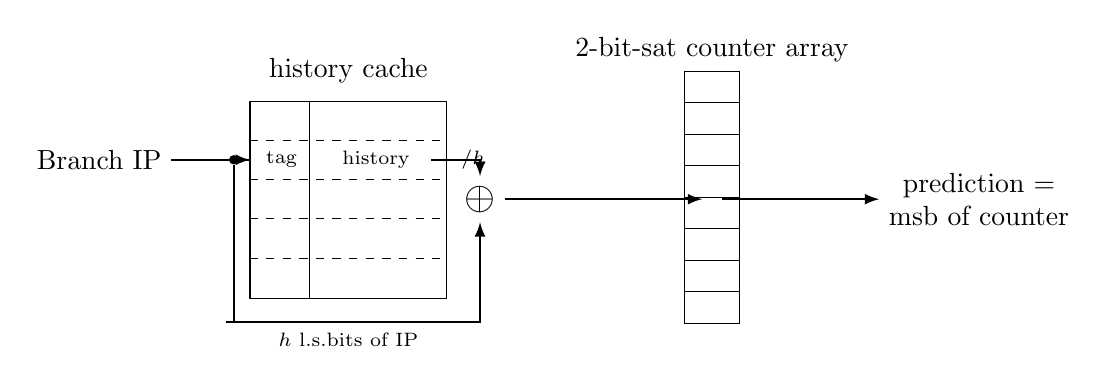
\begin{tikzpicture}[
      box/.style={draw, minimum height=0.8cm, minimum width=1.5cm},
      bigbox/.style={draw, minimum height=2.5cm, minimum width=2cm},
      arrow/.style={-latex, thick},
      data_connector/.style={circle, fill=black, inner sep=1.2pt}
    ]
      % History cache - draw outer box first to reference it
      \node[bigbox, minimum width=2.5cm, minimum height=2.5cm] (hist_cache) at (3,0) {};
      \node[above=0.1cm of hist_cache.north] {history cache};

      % Draw vertical separator line for tag and history columns
      \draw ([xshift=-0.5cm]hist_cache.north) -- ([xshift=-0.5cm]hist_cache.south);

      % Draw horizontal dashed lines for rows
      \foreach \i in {1,2,3,4} {
        \draw[dashed] ([yshift=-\i*0.5cm]hist_cache.north west) -- ([yshift=-\i*0.5cm]hist_cache.north east);
      }

      % Define tag and history box coordinates
      \coordinate (tag_box) at ([xshift=-0.85cm, yshift=-0.75cm]hist_cache.north);
      \coordinate (history_box) at ([xshift=0.35cm, yshift=-0.75cm]hist_cache.north);

      % Add labels in one of the rows (second row)
      \node[font=\scriptsize] at (tag_box) {tag};
      \node[font=\scriptsize] at (history_box) {history};

      % Define tag box entry point (west side of tag cell)
      \coordinate (tag_entry) at ([xshift=-1.25cm, yshift=-0.75cm]hist_cache.north);

      % Branch IP - positioned to the left of tag entry
      \node[left=1cm of tag_entry] (ip) {Branch IP};

      % Data connector circle - to the right of the tag column separator
      \coordinate (separator_line) at ([xshift=-0.5cm]hist_cache.west);
      \node[data_connector] (connector) at ([xshift=0.3cm]separator_line |- tag_box) {};

      % Reference point for history output from east of history box
      \coordinate (history_out) at ([xshift=0.7cm]history_box);

      % XOR operation - positioned even higher
      \node[right=1cm of history_box, yshift=-0.5cm, font=\Large] (xor) {$\oplus$};

      % Calculate coordinates for routing around history cache
      \coordinate (lower_left) at ([xshift=-0.3cm, yshift=-0.3cm]hist_cache.south west);
      \coordinate (lower_right) at ([xshift=0.3cm, yshift=-0.3cm]hist_cache.south east);

      % 2-bit counter array - vertical array
      \node[right=2.5cm of xor] (counter_array_center) {};
      \node[above=1.5cm of counter_array_center] (counter_label) {2-bit-sat counter array};

      % Draw vertical counter array
      \foreach \i in {0,1,2,3,4,5,6,7} {
        \draw ([yshift=-\i*0.4cm]counter_label.south) ++(-0.35cm, 0) rectangle ++(0.7cm, -0.4cm);
      }

      % Prediction output with line break
      \node[right=2cm of counter_array_center, align=center] (prediction) {prediction =\\msb of counter};

      % Arrows
      % Branch IP to tag entry point (west of tag box), then to connector
      \draw[arrow] (ip) -- (tag_entry);
      \draw[thick] (tag_entry) -- (connector);

      % History output from east side going to XOR - using -| pattern with bit width notation
      \draw[arrow] (history_out) -| node[pos=0.2, right, font=\scriptsize] {$/h$} (xor.north);

      % Route from connector around history cache to XOR bottom with bit width notation
      \draw[thick] (connector) |- (lower_left);
      \draw[thick] (lower_left) -- node[midway, below, font=\scriptsize] {$h$ l.s.bits of IP} (lower_right);
      \draw[arrow] (lower_right) -| (xor.south);

      \draw[arrow] (xor) -- (counter_array_center);
      \draw[arrow] (counter_array_center) -- (prediction);
    \end{tikzpicture}
  \end{center}

  \vspace{0.5em}
  \begin{tcolorbox}[colback=green!10, colframe=green!50]
    \centering
    LShare XORs the local history with the branch IP\\
    \small This XOR significantly improves BTB performance
  \end{tcolorbox}
\end{frame}

% Slide 3: Chooser Mechanism
\begin{frame}
  \frametitle{Chooser Mechanism}

  \begin{center}
    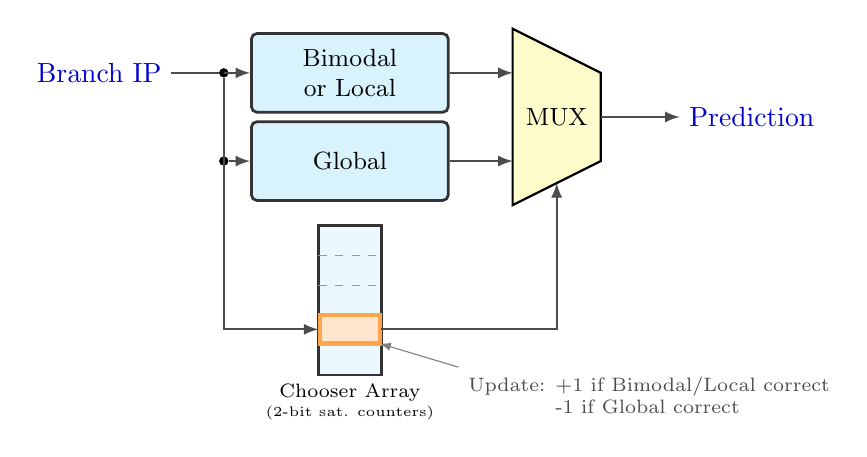
\begin{tikzpicture}[
      box/.style={draw=black!80, line width=1pt, minimum height=1cm, minimum width=2.5cm, fill=cyan!15, rounded corners=2pt, font=\small},
      arrow/.style={-latex, thick, draw=black!70},
      data_connector/.style={circle, fill=black, inner sep=1.2pt}
    ]

      % MUX using circuitikz muxdemux
      \node[muxdemux, muxdemux def={Lh=4, Rh=2, NL=2, NB=1, w=2},
            external pins width=0, fill=yellow!20, anchor=lpin 2] (mux) {};

      % Bimodal or Local box
      \node[box, align=center, left=0.8cm of mux.lpin 1, anchor=east] (bimodal) {Bimodal\\or Local};

      % Branch IP input
      \node[font=\normalsize, text=blue!80!black, left=1cm of bimodal.west] (branch_ip) {Branch IP};

      % Connector for Branch IP
      \node[data_connector, right=0.6cm of branch_ip.east] (conn) {};

      % Global box
      \node[box, left=0.8cm of mux.lpin 2] (global) {Global};

      % Chooser array - drawn with loop and dashed lines, closer to global
      \coordinate (array_start) at ([yshift=-0.3cm]global.south);

      % Draw array box outline - smaller
      \draw[draw=black!80, line width=1pt, fill=cyan!8]
        ([xshift=-0.4cm]array_start) rectangle ++(0.8cm, -1.9cm)
        node[pos=0.5] (chooser_center) {};

      % Draw dashed lines to show array elements - aligned properly
      \foreach \i in {1,2,3,4} {
        \draw[dashed, black!40] ([xshift=-0.4cm, yshift=-\i*0.38cm]array_start) -- ++(0.8cm, 0);
      }

      % Highlight one element in the middle - aligned with dashed lines
      \draw[draw=orange!70, line width=1.5pt, fill=orange!20]
        ([xshift=-0.38cm, yshift=-1.14cm]array_start) rectangle ++(0.76cm, -0.36cm)
        coordinate[pos=1] (highlight_se);

      % Label for chooser array - BELOW the array
      \node[below=0.8cm of chooser_center.south, font=\scriptsize, text=black, align=center, anchor=north]
        {Chooser Array\\[-1pt]\tiny (2-bit sat. counters)};

      % Store chooser position for connections
      \coordinate (chooser_west) at ([xshift=-0.4cm, yshift=-1.32cm]array_start);
      \coordinate (chooser_east) at ([xshift=0.4cm, yshift=-1.32cm]array_start);

      % Label for MUX
      \node at (mux.center) [font=\small] {MUX};

      % Prediction output
      \node[right=1cm of mux.rpin 1, font=\normalsize, text=blue!80!black] (prediction) {Prediction};

      % Arrows - Branch IP to all three components
      \draw[thick, draw=black!70] (branch_ip) -- (conn);
      \draw[arrow] (conn) |- (bimodal.west);
      \node[data_connector] (conn2) at (conn |- global.west) {};
      \draw[thick, draw=black!70] (conn) -- (conn2);
      \draw[arrow] (conn2) -- (global.west);
      \draw[arrow] (conn) |- (chooser_west);

      % Arrows - from predictors to MUX
      \draw[arrow] (bimodal.east) -- ++(0.3, 0) |- (mux.lpin 1);
      \draw[arrow] (global.east) -- ++(0.3, 0) |- (mux.lpin 2);

      % Arrow - Chooser to MUX control (bottom pin)
      \draw[arrow] (chooser_east) -| (mux.bpin 1);

      % Arrow - MUX to Prediction
      \draw[arrow] (mux.rpin 1) -- (prediction);

      % Add update explanation right below the highlighted box
      \node[anchor=north west, font=\scriptsize, text=black!70, align=left] (update_text)
        at ([xshift=1cm, yshift=-0.3cm]highlight_se) {
        Update: +1 if Bimodal/Local correct\\
        \phantom{Update: }-1 if Global correct
      };

      % Arrow from text to highlighted box
      \draw[-latex, draw=black!50, thin] (update_text.north west) -- (highlight_se);

    \end{tikzpicture}
  \end{center}

  \vspace{0.3em}

  \begin{itemize}\small
    \item The chooser selects which predictor to use via the MUX
    \item Each counter tracks which predictor performs better for that branch
    \item The chooser may also be indexed by the Global History Register (GHR)
  \end{itemize}
\end{frame}

% Slide 4: Example Program
\begin{frame}[fragile]
  \frametitle{Example: Nested Loop with Switch}
  
  \begin{tcolorbox}[colback=gray!5, colframe=gray!50]
    \small\ttfamily
    \begin{tabbing}
    \hspace{1em}\=\hspace{1em}\=\hspace{1em}\=\hspace{1em}\=\kill
    for (i=100; i>0; i--)\tikzmark{br0} \textcolor{blue}{$\leftarrow$ Branch 0}\\
    \> for (j=2; j<6; j++)\tikzmark{br1} \textcolor{blue}{$\leftarrow$ Branch 1}\\
    \> \> switch (i\%j) \{ \\
    \> \> \> case 0: ...\tikzmark{br2} \textcolor{blue}{$\leftarrow$ Branch 2}\\
    \> \> \> case 1: ...\tikzmark{br3} \textcolor{blue}{$\leftarrow$ Branch 3}\\
    \> \> \> case 2: ...\tikzmark{br4} \textcolor{blue}{$\leftarrow$ Branch 4}\\
    \> \> \> case 3: ...\tikzmark{br5} \textcolor{blue}{$\leftarrow$ Branch 5}\\
    \> \> \> case 4: ...\tikzmark{br6} \textcolor{blue}{$\leftarrow$ Branch 6}\\
    \> \> \}
    \end{tabbing}
  \end{tcolorbox}
    
\end{frame}

% Slide 5: Branch Behavior Patterns
\begin{frame}
  \frametitle{Branch Behavior Patterns in the Program}
  
  \scriptsize
  
  \begin{tcolorbox}[colback=gray!5, colframe=gray!50]
    \textbf{Branch 0:} TTTT...TTTN (mostly taken, rarely not taken) \\
    \vspace{0.2em}
    \textbf{Branch 1:} TTTNTTTNTTTNTTT... (periodic pattern with N)\\
    \vspace{0.2em}
    \textbf{Branch 2:} TTTTNTTTTNTTNTN... (more complex pattern)\\
    \vspace{0.2em}
    \textbf{Branch 3:} NNNNTTTTNTTTTNTT... (mixed pattern)\\
    \vspace{0.2em}
    \textbf{Branch 4:} TTTTTNNNTTTTTTTT... (clusters of N within T)\\
    \vspace{0.2em}
    \textbf{Branch 5:} TTTTTTTTTTNNTTT... (mostly T with occasional N)\\
    \vspace{0.2em}
    \textbf{Branch 6:} TTTTTTTTTTTTTTTN... (almost always taken)
  \end{tcolorbox}
  
  \normalsize
  \vspace{0.5em}
  Key observations:
  \begin{itemize}
    \item Different branches exhibit different patterns
    \item Some branches have regular patterns (0, 6)
    \item Others have complex, hard-to-predict patterns (2, 3)
    \item Pattern complexity affects prediction accuracy
  \end{itemize}
\end{frame}

% Slide 6: Performance Comparison
\begin{frame}
  \frametitle{Prediction Accuracy Comparison (5-instruction history)}
  
  \begin{columns}[T]
    \column{0.5\textwidth}
    \footnotesize
    \begin{tabular}{|l|c|}
      \hline
      \textbf{Predictor Type} & \textbf{Avg Accuracy} \\
      \hline
      \textcolor{blue}{2-bit counter} & \textcolor{blue}{76.7\%} \\
      Global history \& table & 79.9\% \\
      Local history, global table & 82.9\% \\
      Local history \& tables & 82.1\% \\
      \textcolor{red}{Global history, local tables} & \textcolor{red}{\textbf{83.5\%}} \\
      \hline
    \end{tabular}
    
    \vspace{0.5em}
    \footnotesize
    \textbf{Best performer:} Global history with local tables
    
    \column{0.5\textwidth}
    \begin{center}
      \textbf{Per-Branch Accuracy}\\[0.5em]
      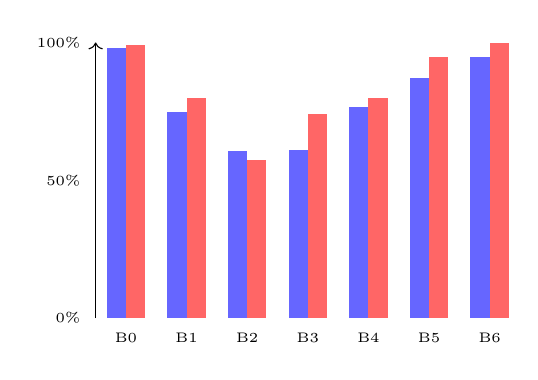
\begin{tikzpicture}[scale=0.7]
        % Draw bars for comparison
        \foreach \branch/\simple/\local in {
          0/98/99,
          1/74.75/79.75,
          2/60.5/57.25,
          3/61/74,
          4/76.75/79.75,
          5/87.25/94.75,
          6/94.75/99.75
        } {
          % Simple predictor bar
          \fill[blue!60] (\branch*1.1, 0) rectangle (\branch*1.1+0.35, \simple/20);
          % Local predictor bar
          \fill[red!60] (\branch*1.1+0.35, 0) rectangle (\branch*1.1+0.7, \local/20);
          % Branch label
          \node[below] at (\branch*1.1+0.35, -0.1) {\tiny B\branch};
        }
        % Y-axis
        \draw[->] (-0.2, 0) -- (-0.2, 5);
        \foreach \y in {0,50,100} {
          \node[left] at (-0.3, \y/20) {\tiny \y\%};
        }
      \end{tikzpicture}
    \end{center}
  \end{columns}
\end{frame}

% Slide 7: Performance Metrics
\begin{frame}
  \frametitle{Performance Metrics}
  
  \begin{center}
    \footnotesize
    \begin{tabular}{|l|c|c|c|}
      \hline
      \textbf{Configuration} & \textbf{Hit Rate} & \textbf{Cycles} & \textbf{Speedup} \\
      \hline
      All wrong & 0.0\% & 1,600,005 & baseline \\
      2-bit counter & 79.0\% & 1,126,005 & 1.42$\times$ \\
      Global history & 79.9\% & 1,120,842 & 1.43$\times$ \\
      Local hist, global table & 82.9\% & 1,102,434 & 1.45$\times$ \\
      Local hist \& tables & 82.9\% & 1,102,434 & 1.45$\times$ \\
      Global hist + local table & 83.5\% & 1,098,594 & 1.46$\times$ \\
      Perfect & 100.0\% & 1,000,005 & 1.60$\times$ \\
      \hline
    \end{tabular}
  \end{center}
  
  \vspace{1em}
  
  \begin{tcolorbox}[colback=yellow!10, colframe=yellow!50]
    \textbf{Test Parameters:}
    \begin{itemize}
      \item Instructions: 1,000,000
      \item Pipeline length: 5
      \item Misprediction penalty: 3 cycles
      \item Branch probability: 20\%
    \end{itemize}
  \end{tcolorbox}
  
  \textbf{Key Insight:} Even modest improvements in prediction accuracy (76\% → 81\%) yield significant performance gains
\end{frame}

\end{document}